%%%% 第一版 2020.10
%此文档为普通物理实验三林伟华老师要求的物理实验报告模板
%作者:武汉大学物理科学与技术学院18级詹睿知
%参考自电子信息学院实验报告模板
%%%% 第二版 2022.8
%更改优化了documentclass
\documentclass{WHUReport}
\usepackage[]{amsmath}
\usepackage{natbib}
\setcitestyle{numbers,square}
\usepackage{amsmath}
\usepackage{esint}

%%%% 以下填写学生信息及实验题目
\newcommand{\major}{物理学}
\newcommand{\name}{郑卜凡}
\newcommand{\stuid}{2021302022016}
\newcommand{\Name}{Bufan Zheng}
\newcommand{\course}{普通物理实验三}
\newcommand{\newtitle}{静电场的测绘}
\newcommand{\Title}{Mapping of Electrostatic Fields}

\begin{document}
\pagestyle{maincontent} 
%\bibliographystyle{plain}

\begin{center}
\zihao{-2} \textbf{\newtitle}\\
\zihao{7}~\\
\zihao{4} \kaishu \name \ \ (\stuid)\\
\zihao{5} \kaishu (武汉大学物理科学与技术学院,湖北省 武汉市 430072)\\
\end{center}
\zihao{-5}\textbf{摘\quad 要:}
%在此处修改中文摘要
本实验利用电流场模拟静电场,对两种不同的面电荷分布的静电场进行了测绘,并且与COMSOL软件建模结果进行了比较,同时定量研究了点电荷电场强度的平方反比律。\\
\zihao{-5}\textbf{关键词:}电流场,静电场,电场线,等势线,Matlab,Comsol。
~\\
\begin{center}
	\zihao{3}\textbf{\Title}\\
	\zihao{-4} \Name\quad (\stuid)\\
	\zihao{5} School of physical science and technology, Wuhan University, Wuhan, 430072, China
\end{center}

\zihao{5}\textbf{Abstract:}In this experiment, current field is used to simulate electrostatic field, and the electrostatic field of two different surface charge distributions is mapped and compared with the modeling result of COMSOL software. Meanwhile, the inverse square law of point charge electric field intensity is quantitatively studied.

\zihao{5}\textbf{Keywords: }Current field, electrostatic field, electric field line, equipotential line, Matlab, Comsol.

\begin{multicols}{2}
	带电体在周围空间中能产生电场,电场强度本身是矢量,但,势$U$为标量,两者之间关系为$\mathbf{E}=-\nabla U$,所以对电场本身的描述可以转化为对电势的描述。但对静电场中的各点进行电势的测量又是十分困难的,因为静电场不会产生电流,因此不能用电流表直接进行测量,若采用静电式仪表测量,则其金属制的探头又会导致原静电场的重新分布,用稳恒电流场模拟静电场的实验设计,使静电场的实验研究比较容易进行,而且这种模拟还可以进一步推广到对温度场的模拟\upcite{ref1,ref2}。
	
	本次实验使用电流场模拟静电场,不同形状的电极给出了不同电荷分布,从而给出了不同的静电场分布,通过对等势线的描绘,便能定性地对静电场进行研究。目的是更好的理解电场线和等势线地相关性质,对常见电荷分布的电场分布有所了解。虽然本实验是定性实验,对于比较简单的点电荷分布,实验者还定量研究了场强随距离的变化。
	\section{实验原理}
	微分方程理论告诉我们, 在一个稳定与时间无关的场中, 若泛定方程与边界条件一旦确定, 则它们的解是唯一确定的。由此可得 出结论, 两个不同性质的 物理场,若描述它们的泛定方程和边界条件相同, 则它们的 解是一一对应的。 进一步讲, 我们若对一种易于测量的场进行测量并得到准确结果, 则与之对应的 另一物理场也可得知。 因此我们可用恒稳电流场来研究与之对应的静电场、温度场。这里我们对稳恒电流场模拟静电场进行说明,对于温度场的模拟可以查阅文献\upcite{ref1,ref2}。
	
	对于静电场,根据Maxwell方程组的齐次方程,可知在无源区域内电场强度满足积分关系为:
	\begin{equation}
		\oiint \mathbf{E}\cdot d\mathbf{S}=0\quad\oint \mathbf{E}\cdot d\mathbf{l}=0
	\end{equation}
	对于稳恒电流场,电流密度矢量$\mathbf{j}$在无源区域内也满足类似的积分关系:
	\begin{equation}
		\oiint \mathbf{j}\cdot d\mathbf{S}=0\quad\oint \mathbf{j}\cdot d\mathbf{l}=0
	\end{equation}
	
	由此可见静电场和稳恒电流场在各自区域中满足同样的数学规律,所以在相同的边界条件下,会具有相同的解析解。因此,我们可以使用稳恒电流场来模拟静电场。
	
	这一数学解释也可以从物理上电荷产生场的观点加以分析。在导电介质中是没有电流通过的,其中任一体积	元(宏观小、微观大、其内仍包含大量原子)内正负电荷数量相等,没有净电荷,呈电中性。	当有电流通过时,单位时间内流入和流出该体积元内的正或负电荷数量相等,净电荷为零,仍然呈电中性。因而,整个导电质内有电场通过时也不存在净电荷。这就是说,真空中的静电场和有稳恒电流通过时导电质中的场都是由电极上的电荷产生的。事实上,真空中电极上的电荷是不动的,在有电流通过的导电质中,电极上的电荷一边流失,一边由电源补充,在动态平衡下保持电荷的数量不变。所以这两种情况下电场分布是相同的。
	
	比如说无限长圆柱同轴电缆之间的电势,无论是两个圆柱作为导体通以稳恒电流,具有固定的电势差,还是把两者看作是带电体具有相反的电荷密度,最终得到的电势分布均为\upcite{ref3}:
	\begin{equation}
		U=U_0\frac{\ln(r_b/r)}{\ln(r_b/r_a)}
	\end{equation}
	\section{实验步骤}
	将导电微晶上内外两电极分别与直流稳压电源的正负极相连接,电压表正负极分别与同步探针及电源负极相连接,电源电压调到10V,从1V开始,平移同步探针,用导电微晶上方的探针找到等位点后,记录下点的坐标和对应的电位,测出一系列等位点,共测9条等位线,每条等势线上找10个以上的点。然后根据电场线与等位线正交原理,再画出电场线,并指出电场强度方向,得到一张完整的电场分布图。注意要根据电场线的疏密程度反映出电场大小的相对强弱,电场线越密集的地方电场强度越大。而且导体的表面是等电势面,所以最终电场线要垂直于电极边界,而且从正电荷出发,止于负电荷或无穷远处。
	\section{点电荷}
	\subsection{静电场的描绘}
	使用半径较小的圆形电极模拟点电荷的静电场是不错的近似。实验上由于越接近中心,电势的变化越快,测量的相对误差迅速增大,所以本次实验共测量了五组数据,从$1V\sim5V$的等势线,每条等势线上标记九个点。为了使用光滑曲线将其连接,利用Matlab对数据点进行立方曲线插值\upcite{ref6},便得到等势线形状:
	\begin{figure}[H]
		\centering
		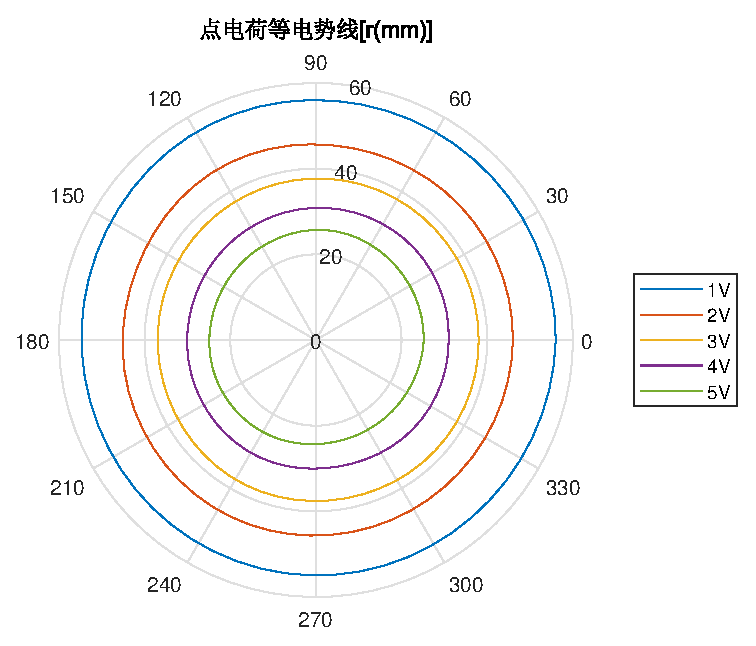
\includegraphics[width=0.85\linewidth]{figs/point_charge.eps}
		\caption{点电荷等势线}
	\end{figure}
	不难看出,等势线是一簇同心圆,而且越往里走越密集。图上也说明了,实验中电极并不严格处于圆心,而是稍有偏离。
	
	根据电场线与等势面垂直,且沿着电场线电势降低的原理,可以绘制出电场线的分布:
	\begin{figure}[H]
		\centering
		\includegraphics[width=0.8\linewidth]{figs/point_e.jpg}
		\caption{点电荷电场线}
	\end{figure}
	\subsection{库仑定律}
	实验中对于$0^\circ$径向上的电势分布进行了测量,得到下图:
	\begin{figure}[H]
		\centering
		\includegraphics[width=0.85\linewidth]{figs/U-R.eps}
		\caption{点电荷电势随距离的分布}
	\end{figure}
	采用径向距离的倒数作为和横坐标绘图,并进行线性拟合:
	\begin{figure}[H]
		\centering
		\includegraphics[width=0.85\linewidth]{figs/U-R-1.eps}
		\caption{$U\mbox{-}\frac{1}{r}$关系}
	\end{figure}
	拟合$R$平方达到了0.98,所以可以得出结论,点电荷的电势与距离成反比,即$U\propto \frac{1}{r}$。此时可以根据$\mathbf{E}=-\nabla U$得到库伦定律,这里我们利用Matlab对数据点进行cubic插值,然后使用中心差分方法近似计算电势相对$r$的一阶导数,绘制得到$E\mbox{-}r$的图像为:
	\begin{figure}[H]
		\centering
		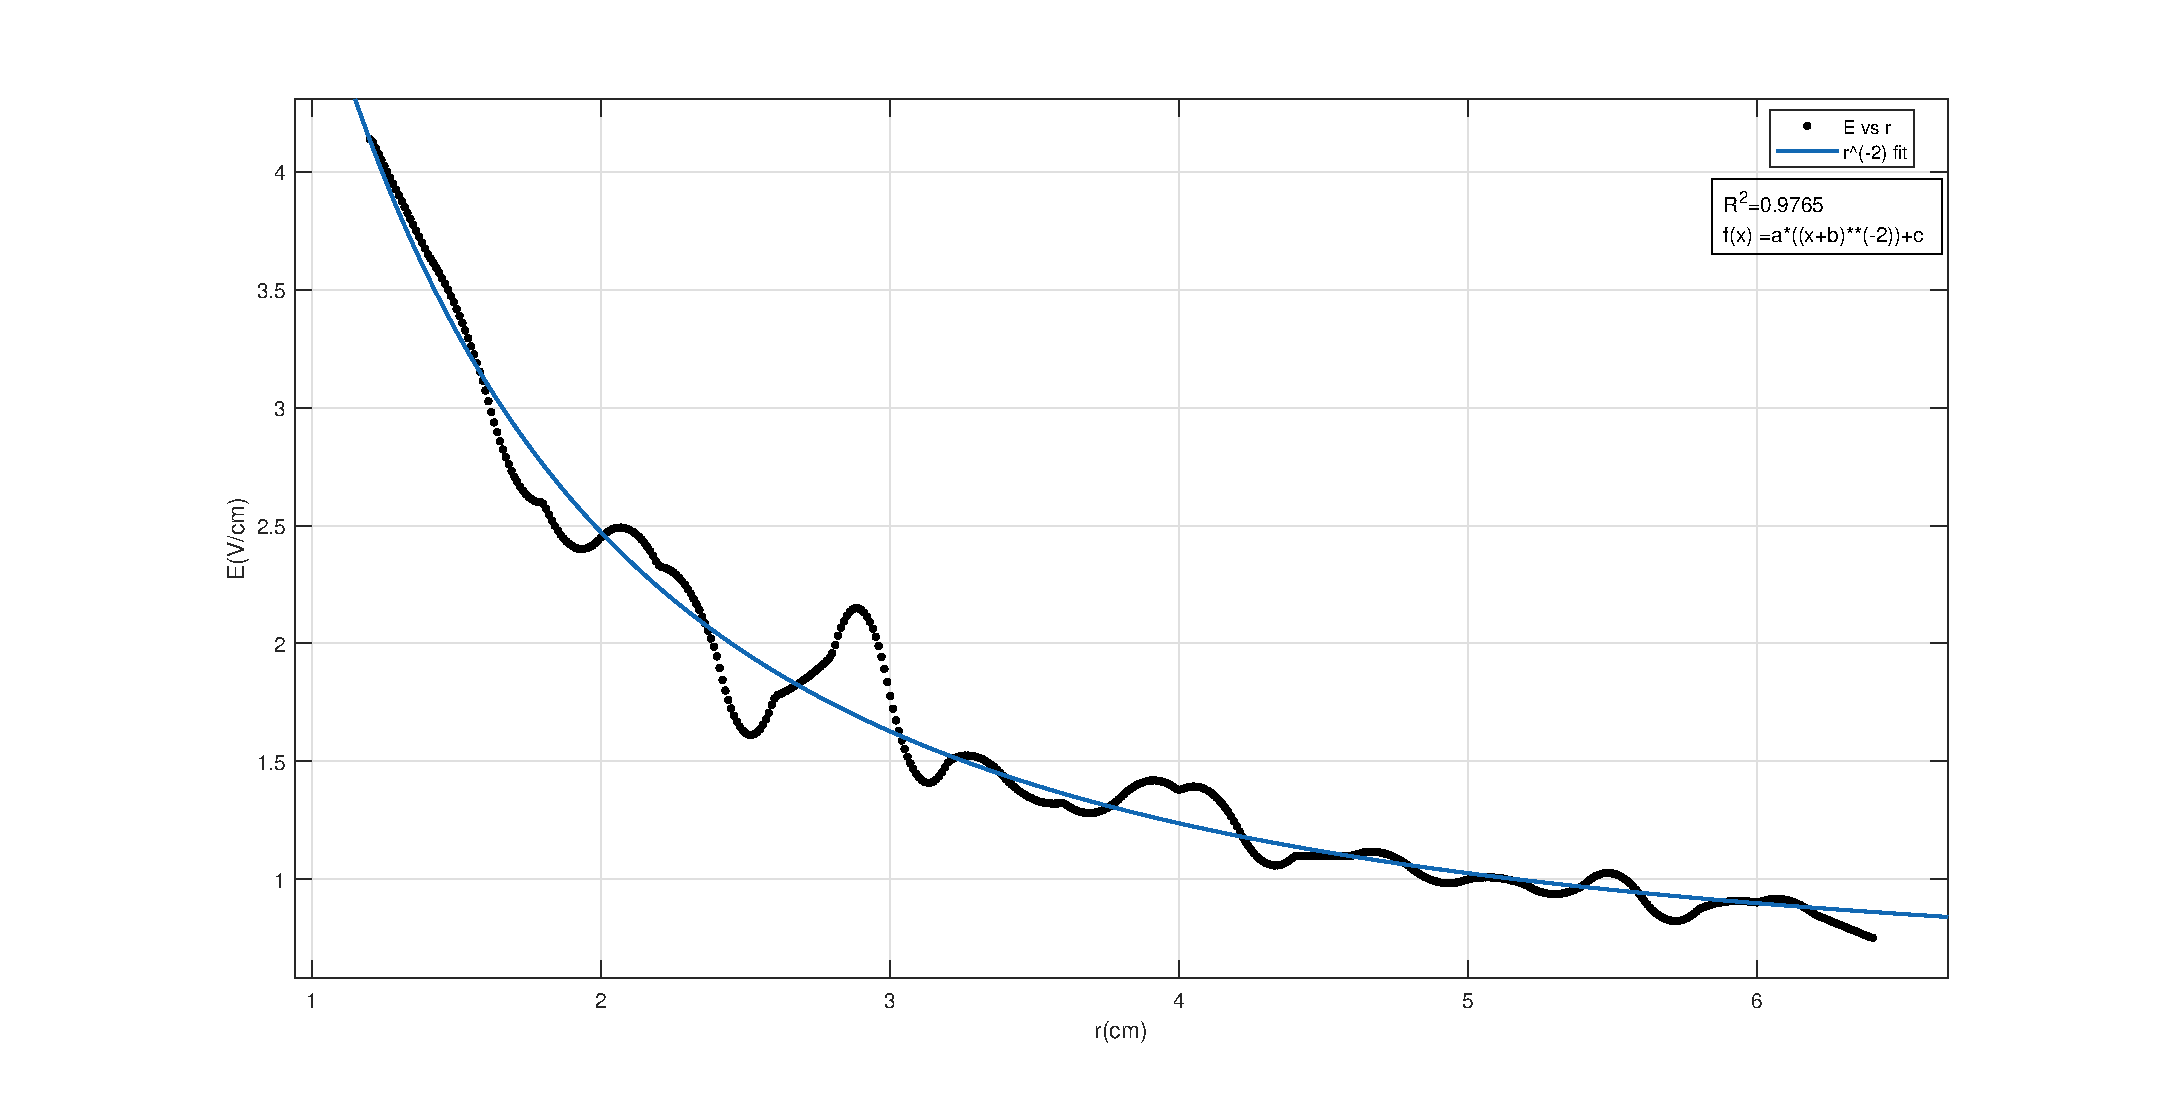
\includegraphics[width=\linewidth]{figs/E-r.eps}
		\caption{$E\mbox{-}r$关系}
	\end{figure}
	其中我们利用$r^{-2}$进行拟合,R平方达到了0.9765,比较精确地验证了库仑定律。受限于插值算法的精度以及测量仪器和测量方法的误差,图上有不少较大的噪声无法消除。
	\section{劈尖电极和条形电极}
	实验还探究了下面的电荷分布的静电场分布:
	\begin{figure}[H]
		\centering
		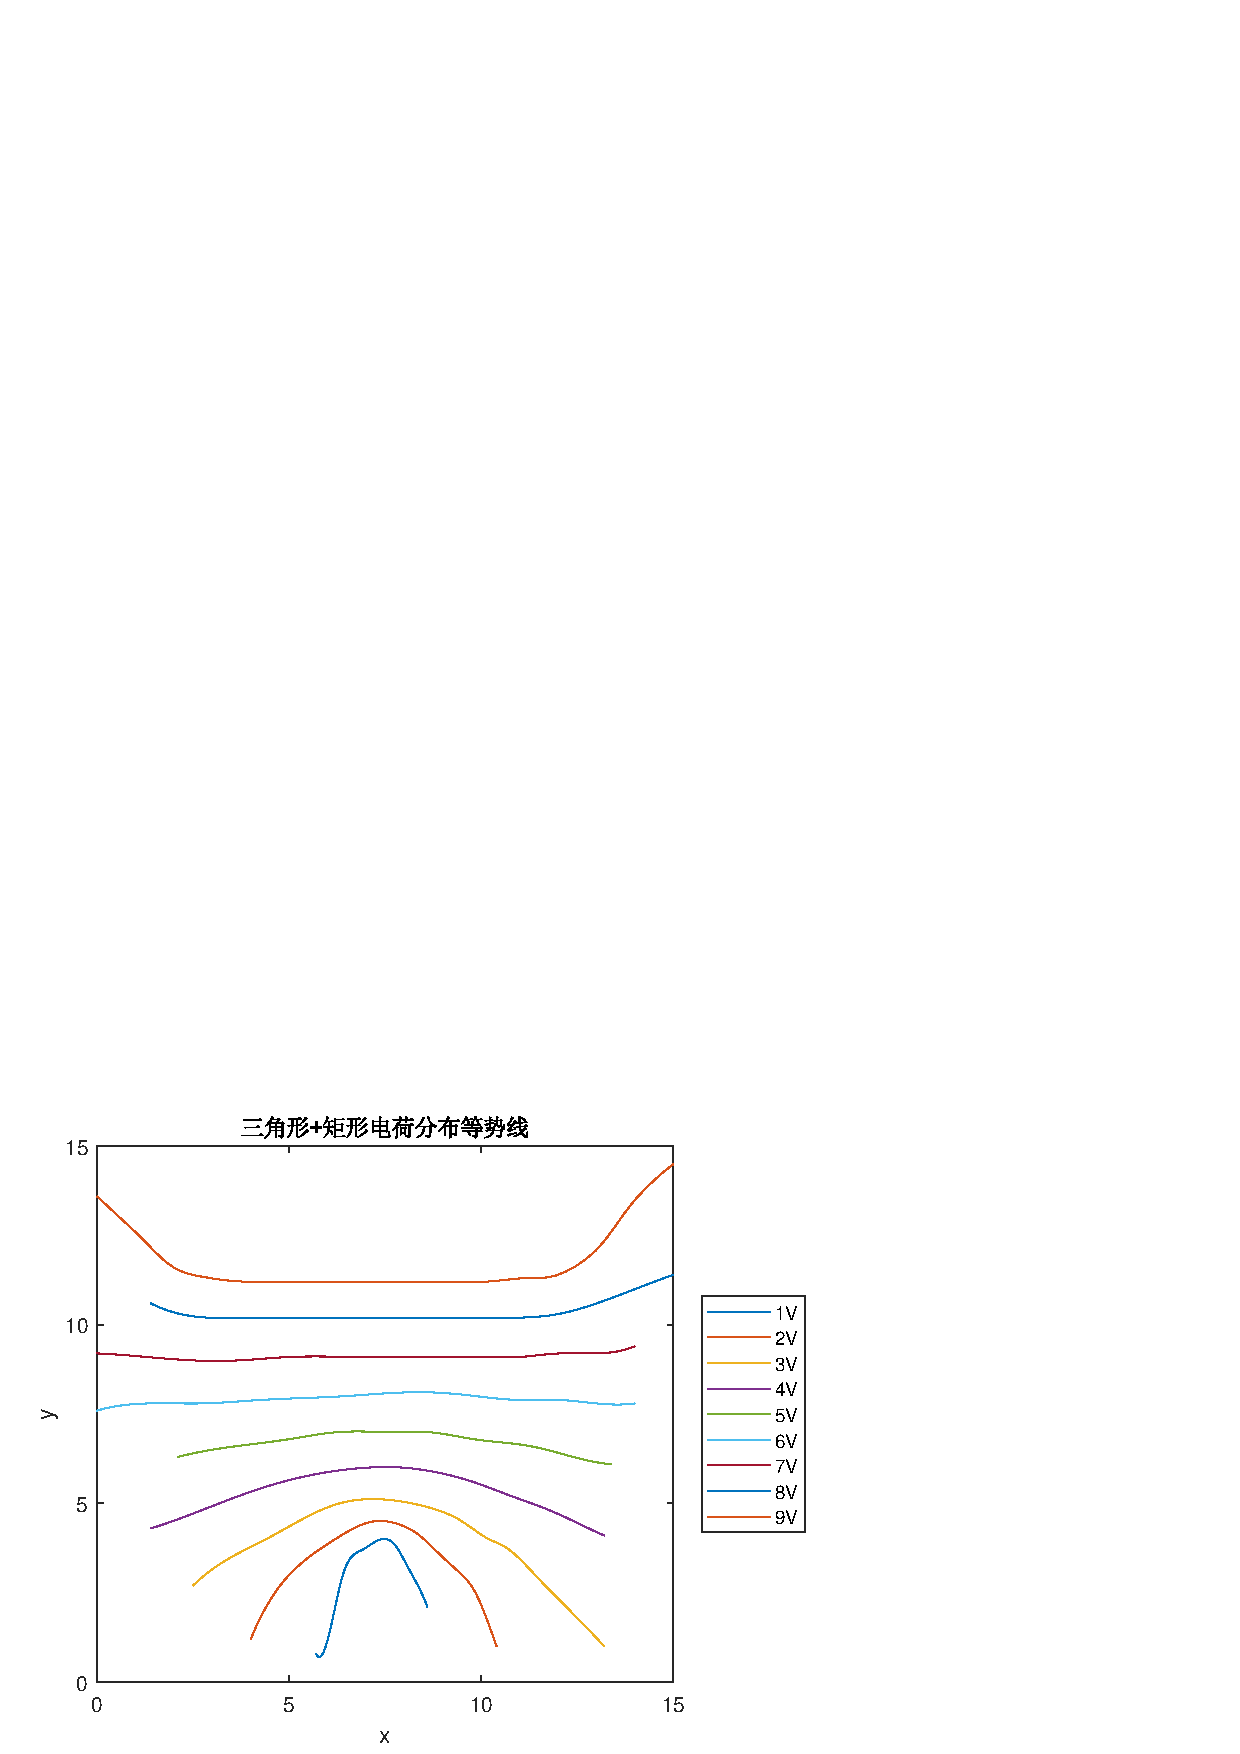
\includegraphics[width=0.85\linewidth]{figs/wedge.pdf}
		\caption{劈尖形电极}
	\end{figure}	
	根据实验数据Matlab插值后得到等势线的平滑曲线如下:
	\begin{figure}[H]
		\centering
		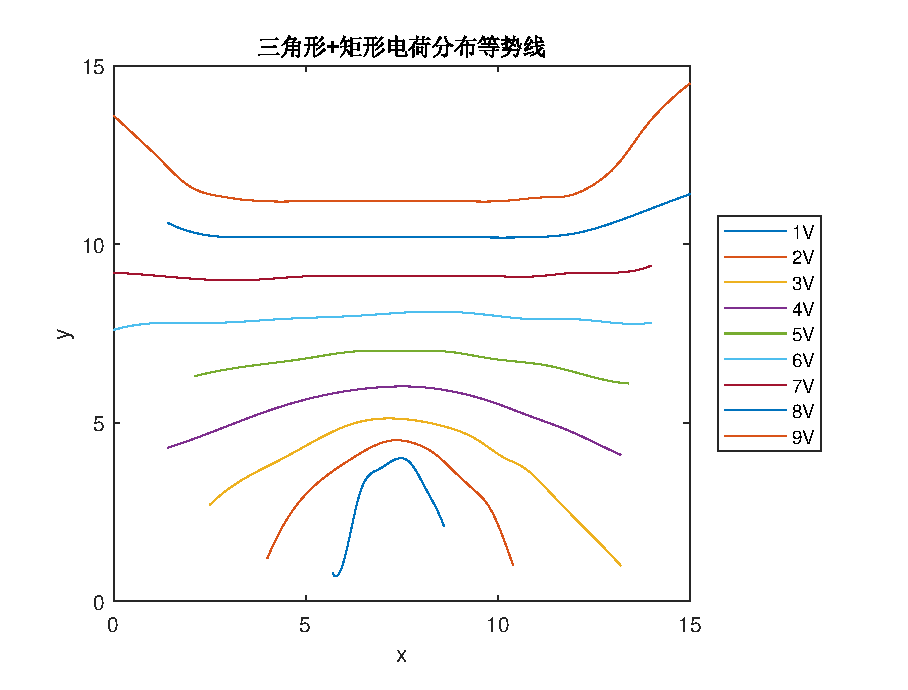
\includegraphics[width=0.85\linewidth]{figs/wedge.eps}
		\caption{劈尖电极和条形电极等势线}
	\end{figure}
	利用绘制点电荷电场线同样的方法,得到下图的电场分布:
	\begin{figure}[H]
		\centering
		\includegraphics[width=0.8\linewidth]{figs/wedge_e.jpg}
		\caption{劈尖电极和条形电极电场线}
	\end{figure}
	利用COMSOL多物理场仿真软件的AC/DC模块对此问题进行静电场稳态建模求解\upcite{ref4,ref5}得到下面的仿真结果:
	\begin{figure}[H]
		\centering
		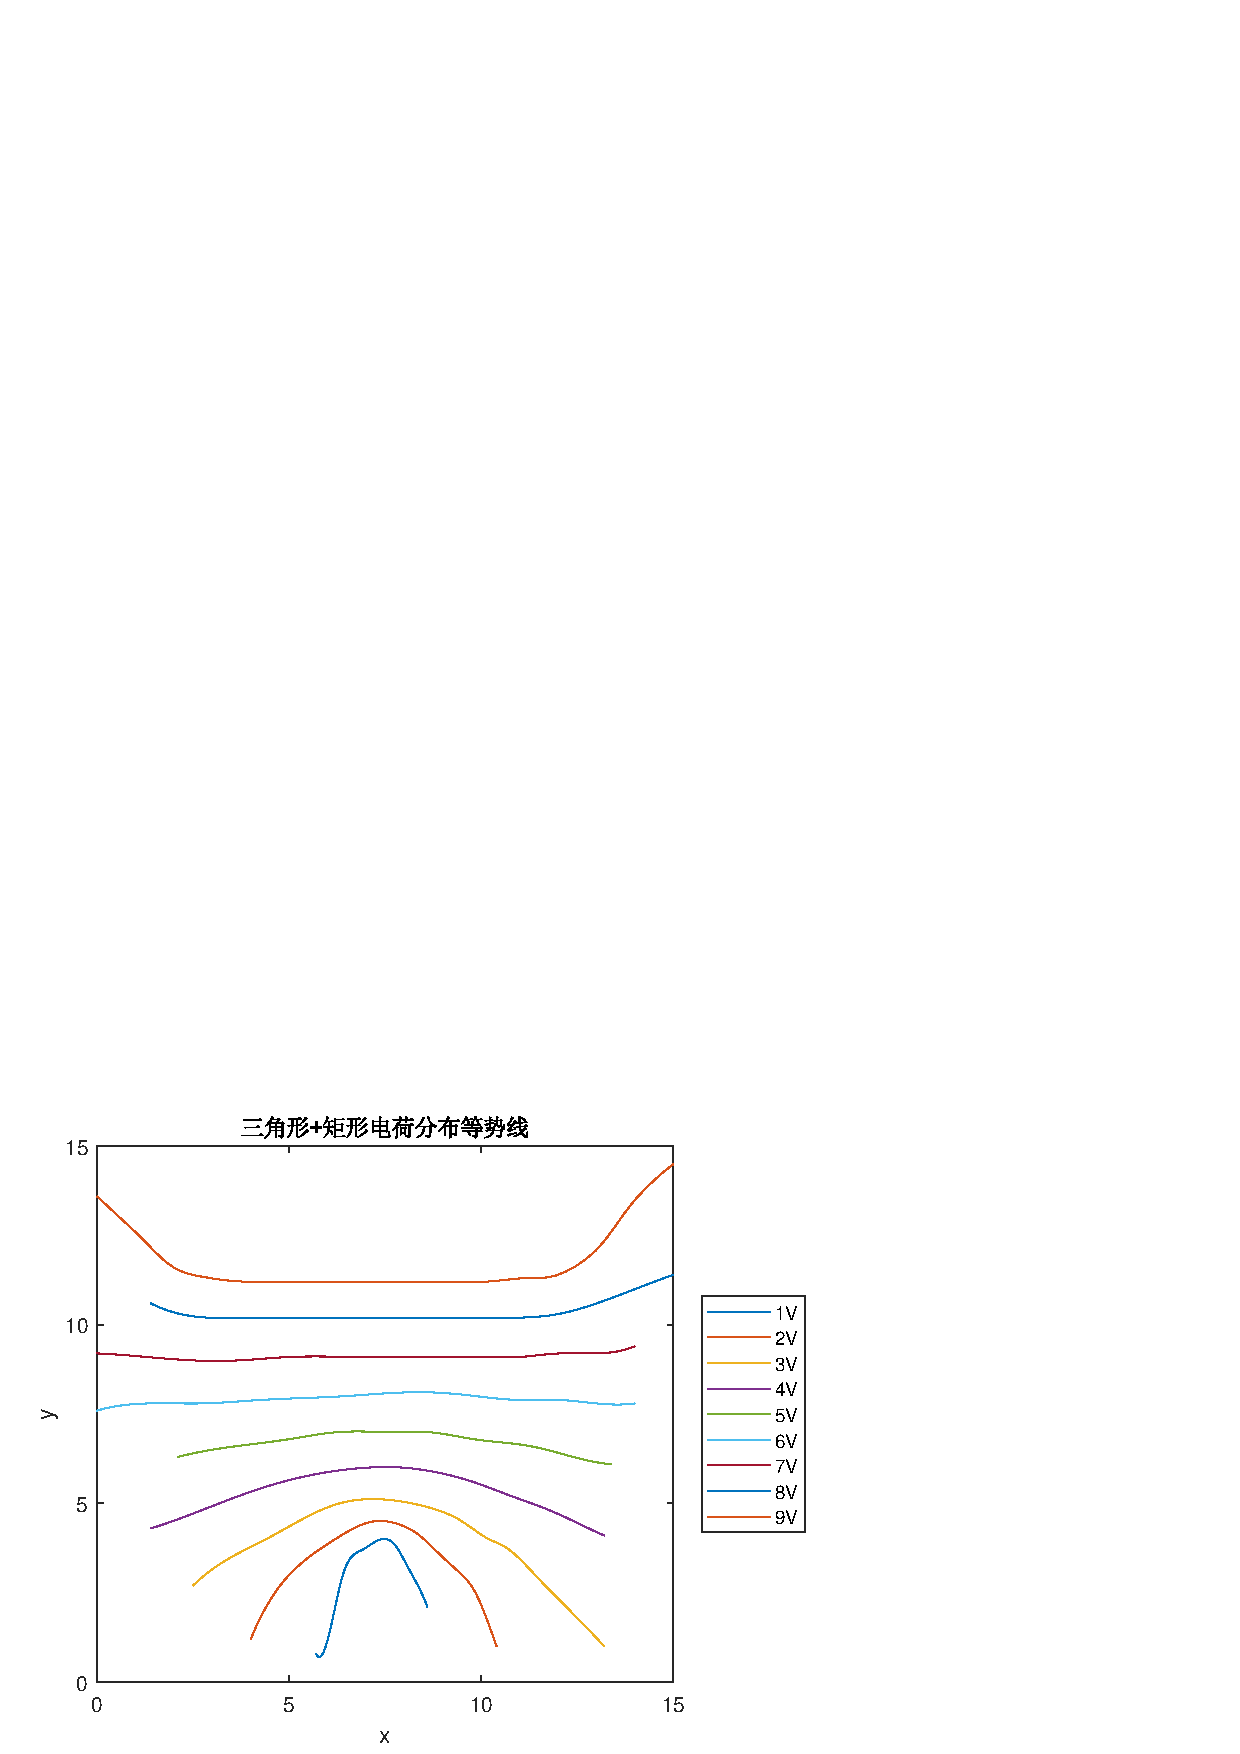
\includegraphics[width=0.85\linewidth]{figs/wedge.png}
		\caption{劈尖电极和条形电极仿真模拟}
	\end{figure}
	比较两者,实验结果在定性上很好的描绘了等电势线和电场线的形状,达到了利用电流场模拟静电场进行实验仿真的要求。
	\section{结\quad 论}
	本次实验利用电流场模拟静电场定性研究了点电荷和劈尖形电荷分布的静电场等势线和电场线形状,并且初步定量的研究了库伦平方反比定律。本次实验收获颇多,首先从原理上掌握了电流场模拟经典场的理论基础,二是在实践中体会了等势线和电场线的一些基础性质,三是学会了使用Matlab进行数据插值处理数据和非线性拟合,最后是熟悉了如何使用COMSOL软件对静电场问题进行建模求解分析。
	
	当然,本次实验在数据处理方面还有些地方待以改进,比如在得到等势线之后根据电场线与等势线原理绘制电场线是直接手工绘制的,并没有实现软件自动化绘制。这或许可以在等势线测得比较密集之后进行插值,然后机器计算与等势线相交垂直的曲线并进行绘制。这是本实验可以改进拓展研究的地方,由于时间原因没有来得及进行探究。
	\bibliographystyle{unsrt}
	\begin{thebibliography}{99}  
		\bibitem{ref1}陈新雷,乔卫平.用模拟法测绘流场和温度场[J].物理实验,1995(02):57-59.
		\bibitem{ref2}[1]陈新雷,乔卫平.用模拟法测绘二维流场和温度场[J].工科物理,1994(03):21-23.
		\bibitem{ref3}赵凯华,陈熙谋.电磁学[M].4版,北京:高等教育出版社,2018.
		\bibitem{ref4}曾鑫,闫向宏,张亚萍.利用有限元数值模拟技术辅助静电场学习[J].物理与工程,2020,30(05):87-91.
		\bibitem{ref5}杨军鹏,安小宁.基于COMSOL Multiphysics的静电场仿真分析[J].物理通报,2020(01):99-100+103.
		\bibitem{ref6}戚非,韩瑞萍.物理实验数据的多项式拟合与插值[J].大连大学学报,2004(06):19-21.
	\end{thebibliography}
\end{multicols}

\end{document}
